{\color{indiagreen}\subsection{Delo in mehanska energija}}
\begin{align*}
	A &= Fs [1Nm = 1J]\\
\end{align*}
A \dots delo\\
s \dots premik prijemališča sile\\
Velja samo v primeru, ko je sila konstantna in je premik prijemališča vzporeden sili.\\
\begin{center}
	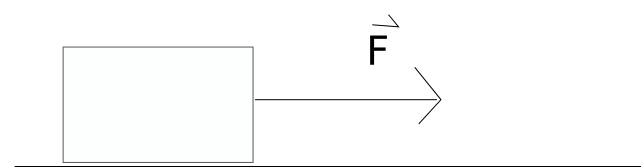
\includegraphics[width=15cm, height=15cm,keepaspectratio=true]{delo.png}
\end{center}
$F = konst.$ \hspace{1cm} $\vec{F} || \vec{s}$\\
\begin{align*}
	A &= \vec{F} x \vec{s} = Fs\cos\alpha\\
\end{align*}
\begin{center}
	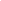
\includegraphics[width=15cm, height=15cm,keepaspectratio=true]{Delo2.png}
\end{center}
$A = 0$\\
\begin{center}
	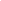
\includegraphics[width=15cm, height=15cm,keepaspectratio=true]{Delo3.png}
\end{center}
$A < 0$\\
\begin{center}
	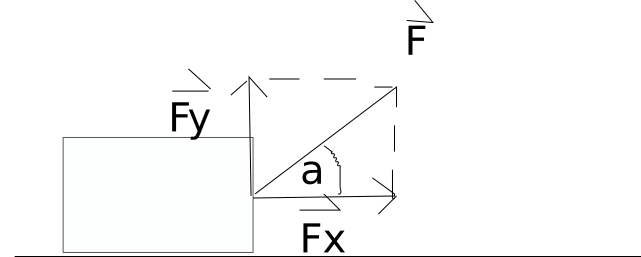
\includegraphics[width=15cm, height=15cm,keepaspectratio=true]{Delo4.png}
\end{center}
\begin{align*}
	A &= \vec{F_x} x \vec{s} = Fs\cos\alpha\\
\end{align*}
\begin{center}
	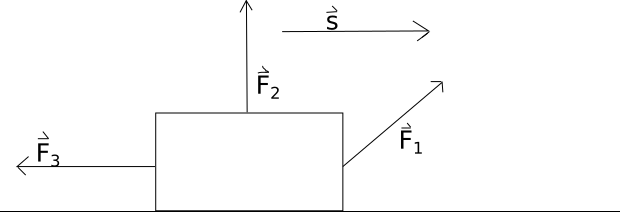
\includegraphics[width=15cm, height=15cm,keepaspectratio=true]{Delo5.png}
\end{center}
\begin{align*}
	A &= A_1 + A_2 + A_3 = F_xs + 0 - F_3s\\
\end{align*}
